\chapter{Conceptual framework}
\label{chap:conceptual}

As a first step we review the tools and concepts needed for our discussion, which will rest on three fundamental pillars: how we handle information, how quantum systems are described and which type of schemes are useful for quantum metrology. 

\section{Fundamentals I: probability theory}
\label{sec:probability}

Our main aim is to study how quantum metrology protocols are to be designed when the finite character of the number of observations is explicitly taken into account, with a particular emphasis on the regime of limited data. In this context it is natural to employ a formulation of probability theory where the central focus lies on the information content of our probabilities, and this is precisely the path that we will follow. The formal elements of this approach, which can be seen as a part of the Bayesian paradigm \cite{jaynes2003}, are briefly reviewed in the following sections\footnote{The Bayesian framework can also be constructed using bets, profit and degrees of belief \cite{definetti1990, bernardo1994}. Here we do not follow this subjectivist approach because metrology rests on the study of natural phenomena, and this is an impersonal enterprise. One may also work with a purely measure-theoretic version of the theory \cite{rosenthal2006} if the problem can be recast in the language of sets, although this is not always possible when the prior information acquires an important role \cite{jaynes2003}. Finally, note that a definition of probabilities in terms of relative frequencies that arise in a repeated experiment is not appropriate for us, since the regime of limited data includes, by definition, scenarios where the number of trials is low, or where some events happen only once. Moreover, note that it can be consistently argued that probabilities and relative frequencies are conceptually different quantities, where the former are assigned by us or by our theory and the latter are empirical facts (see \cite{jaynes2003, jeffreys1961, jiangwei2014}, and also our discussion in section \ref{subsec:lln}).}. 

\subsection{Calculus of probabilities}
\label{subsec:calprob}

Following the expositions given by Ballentine \cite{ballentine1998}, Van Horn \cite{vanhorn2003} and Jaynes \cite{jaynes2003}, we can capture the rules of probability theory using the following axioms:
\begin{enumerate}
\item $0 \leqslant P(A|B) \leqslant 1$,
\item $P(A|B) = 1$ when it can be concluded that $A$ is true on the basis of $B$,
\item $P(\neg A | B) = 1 - P(A | B)$, and
\item $P(A \land B | C) = P(A | C) P(B |A \land C)$,
\end{enumerate}
where $A$, $B$ and $C$ are propositions, and the symbols $\neg$ and $\land$ are the connectives for negation and conjunction, respectively \cite{nidditch1962, copi2016}. The probability $P(A|B)$ is to be understood as the degree of plausibility for $A$ to be true given $B$, and it can be seen as a carrier of information. More concretely, $B$ encodes either what is known about the real world or hypotheses about it, i.e., it represents a state of information \cite{jaynes2003, vanhorn2003}, and the logical analysis of this information is what determines the plausibility associated with the proposition $A$, which is the object of our enquiry. The two extremal values of the scale of plausibility correspond to the most informative scenarios, which recover as particular cases the two truth values found in propositional logic \cite{jaynes2003, nidditch1962, copi2016}, while any other intermediate plausibility will be associated with an uncertain scenario. Thus probability theory is seen as an extension of propositional calculus that allows us to encode and manipulate information in uncertain situations\footnote{There has been some debate as whether the word \emph{plausibility} should be employed as it is done here \cite{shafer2004, vanhorn2004}, since this word is used in a different sense in the theory of belief functions \cite{shafer2004}. Nevertheless, it can be argued that, historically, its use in our context is older \cite{vanhorn2004}, and we have found that, in practice, it is particularly convenient for studying estimation problems, which is our topic of discussion.} \cite{jaynes2003}. 

This way of understanding probabilities can be justified via Cox's work \cite{cox1946, cox1961}, provided that his assumptions for a reasonable measure of plausability are accepted. There is a rich literature about the validity, scope and limitations of this approach \cite{paris1994, vanhorn2003, colyvan2004, clayton2017, vanhorn2017}, but for our purposes suffice it to say that: i) there exists a rigorous treatment of Cox's ideas (see \cite{paris1994}), and (ii) in practice it can be successfully applied to a wide range of real-world problems, as the work of authors such as Jeffreys \cite{jeffreys1961} and Jaynes \cite{jaynes2003} demonstrates.

Two important concepts are those of mutual exclusivity and independence \cite{jaynes2003}. Mutually exclusive propositions satisfy that $P(A_1 \lor \cdots \lor A_s | I_0) = \sum_{i=1}^s P(A_i | I_0)$, where $\lor$ indicates disjunction \cite{nidditch1962, copi2016}, and we have that $\sum_{i=1}^s P(A_i | I_0) = 1$ if $\lbrace A_i \rbrace$ are also exhaustive. In addition, independence is expressed as $P(B_1 \land \cdots \land B_r | I_0) = \prod_{j=1}^r P(B_j | I_0)$. Beyond these notions, for us the key result that can be derived from these axioms is Bayes theorem: 
\begin{equation}
P(A | B \land I_0) = \frac{P(A | I_0) P(B | A \land I_0)}{P(B | I_0)},
\label{bayestheorem1}
\end{equation}
where $P(B | I_0) = P(A | I_0 ) P(B |A  \land I_0 ) + P(\neg A | I_0 ) P[B |(\neg A) \land I_0]$. 

To understand equation (\ref{bayestheorem1}), suppose we take $A$ to be a proposition about theoretical parameters, and imagine that the experimental outcomes are encoded in $B$. Furthermore, $I_0$ represents our initial state of information, which in this case includes the conditions under which the experiment is performed and the possible ranges for parameters and outcomes\footnote{In quantum metrology we can think of the prior information $I_0$ as a formal representation of the operational information that indicates how the experiment is to be arranged and performed, which in general is a collection of instructions expressed in the language of experimental physics.}. Then we can see that, according to equation (\ref{bayestheorem1}), the prior probability $P(A | I_0)$ is updated using the new information about $A$ provided by the empirical evidence $B$, which is encoded in the likelihood $P(B | A \land I_0)$, and the denominator acts as a normalisation constant. The overall result is the construction of the posterior probability $P(A | B \land I_0)$, which gives us the plausibility for $A$ to be true given the prior information $I_0$ and the empirical data $B$. 

When the propositions refer to variables, as it is the case of $A$ and $B$ in the previous example, probabilities are defined in term of certain probability functions that act as mathematical models for the information about the situation under analysis. For example, 
\begin{equation}
P(\Delta_{\theta'}| I_0) \equiv P(\theta \in \Delta_{\theta'}| I_0) = \int_{\Delta_{\theta'}} d\theta'' ~p(\theta'') 
\label{cont1}
\end{equation}
is the probability that $\theta$ lies in an interval of boundaries $\theta'$ and $\theta' + \Delta_{\theta'}$, where we have introduced the probability density function $p(\theta)$. In a similar way,
\begin{equation}
P( \Delta_{\theta'} \land \Delta_{m'} | I_0 ) = \int_{\Delta_{\theta'}} d\theta'' \int_{\Delta_{m'}} dm''~p(\theta'', m''),
\label{cont2}
\end{equation}
where $p(\theta, m)$ is a joint density. Note that while probabilities are dimensionless numbers, probability densities can have units.  

For the conditional density we may use equations (\ref{cont1}) and (\ref{cont2}), assume that $\Delta_{m'} \ll 1$ and $\Delta_{\theta'} \ll 1$, such that 
\begin{equation}
P( \Delta_{m'} | \Delta_{\theta'} \land I_0 )= \frac{P( \Delta_{\theta'} \land \Delta_{m'} | I_0 )}{P(\Delta_{\theta'}| I_0)} \rightarrow \frac{p(\theta', m')}{p(\theta')}\Delta_{m'},
\end{equation}
and take $p(m|\theta) = p(\theta, m)/p(\theta)$. The linear approximation in the last step can be found by integrating the Taylor expansions of the density functions $p(\theta'', m'')$ and $p(\theta'')$ around $\theta'$ and $m'$. Since this procedure also applies to $P(\Delta_{\theta'} |\Delta_{m'} \land I_0 )$, we have that $p(\theta|m) = p(\theta) p(m|\theta)/p(m)$, with $p(m)=\int d\theta ~p(\theta) p(m|\theta)$. That is, we have a version of Bayes theorem in terms of densities, and the same idea is valid when we consider vector variables. We note that in this thesis we follow the convention of omitting integration limits of general expressions where the integration is taken over the complete parameter domain, as it is the case in the latter integral. 

Sometimes it is useful to employ the more compact notation $P(d\theta| I_0 ) = p(\theta)d\theta$ and $P(d\theta \land dm | I_0) = p(\theta, m)d\theta dm$, which arises from equations (\ref{cont1}) and (\ref{cont2}) by taking infinitesimally small intervals. In general we will use the language of continuous variables because this also includes discrete cases when we allow the densities under our integration symbols to involve sums of Dirac deltas \citep{jaynes2003, breuer2002}. In those cases where an explicitly discrete treatment is more convenient, we will use the notation $P(n = n' | I_0 ) \equiv p(n')$, where $p(n)$ is a probability mass function. 

The previous description is suitable for those variables for which only uncertain information is available. Common reasons for this situation to arise are lack of knowledge, lack of control in an experiment and the existence of fundamental limits that nature imposes. The latter scenario is best illustrated by quantum systems. 

Finally, instead of working with the variables themselves, we often wish to consider some function of them. In that case, a useful quantity to have an idea of the magnitude of such function is the average. For instance, we could have $\bar{f} = \int d\theta dm~ p(m,\theta) f(m, \theta)$. 

\subsection{Law of large numbers}
\label{subsec:lln}

Another important result that we will exploit is the law of large numbers. Given the proposition $B$ representing a physical event generated in an experiment specified in $I_0$, the weak version of this law is \cite{ballentine2016, rosenthal2006} 
\begin{equation}
\lim_{\mu \to \infty} P(\abs{f_\mu - P(B|I_0)} \geqslant \varepsilon~ |I_0) = 0,
\label{lawlargenumbers}
\end{equation}
where $f_\mu = n_B(\mu)/\mu$ is the relative frequency of $B$ after performing $\mu$ independent repetitions of the experiment in $I_0$, and $\varepsilon$ is a positive number. We say that $f_\mu$ converges in probability to $P(B|I_0)$ \cite{rosenthal2006}.

The importance of this result is that it offers an empirical link between probabilities and relative frequencies, since the latter are quantities that we measure in the laboratory. To see why, we propose the following argument. First we recall that $P(B|I_0)$ is the plausibility for the event $B$ to happen when the experiment in $I_0$ is run once. Presumably, $I_0$ encodes the procedure that generates the events, and it also contains the fact that our actions do not produce the same event in each new repetition. The key observation is that $f_\mu$ in equation (\ref{lawlargenumbers}) is based on the same $I_0$, in the sense that we could perform a simulation where $P(B|I_0)$ and $P(\neg B|I_0)$ are used for generating $\mu$ outcomes, and calculate the relative frequency $f_\mu$ for the event $B$ from them. In view of this, equation (\ref{lawlargenumbers}) expresses the intuitive idea that if in each run some outcomes are more (less) likely to appear, then as we increase the number of repetitions it is also likely that the largest (lowest) values for relative frequencies correspond to the largest (lowest) single-shot probabilities.

The frequency $f_\mu$ in the previous discussion is not yet factual, but a prediction made on the basis of $I_0$ and our model $P(B|I_0)$. If we now perform the actual experiment and we observe that the experimental frequencies after a very large number of trials are compatible with those that come from the model, we may think of it as a good representation of the available information about the physical phenomenon that gave rise to the experiment. Moreover, since it is likely that $f_\mu$ and $P(B|I_0)$ are close in the long run, we may also imagine that the experimental frequencies are to be compared to the probability $P(B|I_0)$ directly.

This idea becomes even more meaningful when we consider the strong version of the law, which instead states that $f_\mu \rightarrow P(B|I_0)$ almost surely as $\mu$ increases \cite{rosenthal2006}. Crucially, comparing probabilities and relative frequencies is precisely what is done in practice with quantum experiments. A good example can be found in the results of \cite{baumgart2016} for the implementation of a magnetometer. In particular, this work shows a good agreement between the quantum-mechanical probabilities and the measured frequencies, which is fully compatible with our rationale above. As a consequence, this way of looking at the law of large numbers provides a clear link with experiments while probabilities are still seen as mathematical models that encode information, and that are qualitatively different from the concept of relative frequency. 

\section{Fundamentals II: quantum mechanics}
\label{sec:qmech}

In his celebrated work of 1925 (page 261 of \cite{waerden1967}), Heisenberg offered an insight that would eventually lead to the modern formalism of quantum mechanics. Starting by representing the dynamical variables\footnote{The dynamical variables represent elementary properties that we can use to describe a physical system, and also its variation in time. Examples of these include the positions and momenta of an ensemble of particles, the components of their spin or the amplitude of a field.} with Fourier terms, his key idea was to modify these terms such that the experimental facts of the atomic realm could be accommodated, while still retaining the form of the classical laws of dynamics. As a result, later work built on this premise produced a new formalism broad enough to generate probability models that can capture the behaviour of the phenomenology of quantum systems, whose nonclassical features stem from the discreteness associated with the quantum of action $h$. We turn now our attention to how this theory describes the physical systems that we use in quantum metrology.  

\subsection{Elements of the theory}
\label{subsec:elements}

A useful way of looking at the theory is to decompose it in three parts:
\begin{enumerate}
\item Each dynamical variable is represented with a Hermitian operator whose spectrum contains the real numbers that such variable can take, or the intervals in which it can lie. Physical systems are then characterised by a set $\boldsymbol{Z}(t) = \lbrace Z_1(t), Z_2(t), \dots\rbrace$ of these Hermitian operators, for which
\begin{equation}
\left[Z_i(t),Z_j(t)\right] = Z_i(t)Z_j(t) - Z_j(t)Z_i(t) \neq 0
\label{commutator}
\end{equation}
for at least some of the cases where $i \neq j$. That the Hermitian operators for different dynamical variables may not commute is a mathematical representation of the fundamental limits associated with the existence of $h$.
\item To model more complex aspects of the quantum realm we can construct general functions $f(\boldsymbol{Z}(t), t)$, and we can consider their evolution in time, which for closed systems is given by Heisenberg's equation of motion \cite{englert2013, schwinger2001}
\begin{equation}
\frac{d}{d t} f(\boldsymbol{Z}(t), t) = \frac{\partial}{\partial t}f(\boldsymbol{Z}(t), t) + \frac{1}{i\hbar} \left[f(\boldsymbol{Z}(t), t),H(\boldsymbol{Z}(t), t)\right],
\label{heisenbergeq}
\end{equation}
with initial condition $f(\boldsymbol{Z}(t_0), t_0) = f_0$. The function $H(\boldsymbol{Z}(t), t)$ is the Hamiltonian, a Hermitian operator that generates the temporal displacement, and $\hbar = h/(2\pi)$ is the reduced Planck constant. Note that equation (\ref{heisenbergeq}) also gives the evolution of the dynamical variables themselves when $f(\boldsymbol{Z}(t), t) = Z_i(t)$, for any $i$. Among all the functions $f(\boldsymbol{Z}(t), t)$, two of them play a crucial role in the theory:
\begin{enumerate}
\item[2.i.] The density operator $\rho(\boldsymbol{Z}(t), t)$ is a positive semi-definite Hermitian operator satisfying $\mathrm{Tr}[\rho(\boldsymbol{Z}(t),t)] = 1$, and it represents how the system is prepared at some moment in time \cite{englert2013,ballentine1998}. We call this the state preparation procedure \cite{ballentine1998}, or simply state. When the system is closed, the details of the initial preparation are preserved as time passes, and as such we have that $d\rho(\boldsymbol{Z}(t),t)/dt = 0$ \cite{englert2013, schwinger2001}. Inserting this fact into equation (\ref{heisenbergeq}) we find von Neumann's equation
\begin{equation}
\frac{\partial}{\partial t}\rho(\boldsymbol{Z}(t), t) =  \frac{1}{i\hbar} \left[H(\boldsymbol{Z}(t), t), \rho(\boldsymbol{Z}(t), t)\right],
\label{vonneumann}
\end{equation}
with initial condition $\rho(\boldsymbol{Z}(t_0), t_0) = \rho_0$.
\item[2.ii.] The probability operator
\begin{equation}
E(\Delta_{m'}, \boldsymbol{Z}(t), t) = \int_{\Delta_{m'}} dm''~E(m'', \boldsymbol{Z}(t), t),
\end{equation}
also positive semi-definite and Hermitian, represents a measurement device or instrument \cite{helstrom1976} that interacts with a system described by $\boldsymbol{Z}(t)$, generating an event characterised by an outcome $m$ that lies in some subinterval of width $\Delta_{m'}$. We say that $E(m, \boldsymbol{Z}(t), t)$ generates a probability-operator measurement (POM)\footnote{Also known as positive operator-valued measure (POVM) \cite{englert2013, jiangwei2014, barnett2014}.}, such that the identity is resolved as
\begin{equation}
\int dm~E(m, \boldsymbol{Z}(t), t) = \mathbb{I}.
\end{equation}
\end{enumerate}
\item The Born rule establishes that the probability density for observing the outcome $m$ at time $t$ is given by
\begin{equation}
p(m|t) = \mathrm{Tr}\left[E(m, \boldsymbol{Z}(t), t) \rho(\boldsymbol{Z}(t), t) \right],
\label{bornrule}
\end{equation}
and it provides the link between theory and experiment. In particular, the probability model $p(m|t)$ can be used to predict the relative frequencies that we measure in the laboratory, following the rationale that we discussed in section \ref{subsec:lln} in connection with the law of large numbers.
\end{enumerate}

According to the Born rule, quantum probabilities can be seen as depending on two different types of information. On the one hand, they depend on our choices for the functions $\rho(\cdot)$ and $E(\cdot)$. Following current practice, we will employ rank-one operators such as pure states and projective measurements when, for all practical purposes, the preparation of systems and instruments involves a degree of control so high that can be thought of as to provide maximum information. Otherwise, mixed states (i.e., density operators for which $\mathrm{Tr}[\rho(t)^2]\neq \mathrm{Tr}[\rho(t)] = 1$ \cite{breuer2002}) and more general POMs are to be employed. Note that projective measurements originate in the idea of quantum observable. In particular, an observable is a physical quantity represented by a Hermitian operator whose eigenvectors give rise to a measurement scheme. For example, upon calculating the spectral decomposition $Z(t) = \int dz\,z \ketbra{z,t}$ for the dynamical variable $Z(t)$, we can implement its measurement using the projectors $\ketbra{z,t} = E(z,t)$, for which $ E(z,t)dz E(z',t) dz' = \delta(z - z')E(z, t)dz dz' $. 
 
On the other hand, quantum probabilities also incorporate the nonclassicality that emerges from $h$ via the commutation relations for the dynamical variables, and also through the law of evolution in equation (\ref{heisenbergeq}). That $p(m|t)$ takes into account the relevant role of $h$ in quantum physics offers, in fact, a good way of understanding the success of quantum technologies. Probabilities in classical physics are less constrained because their only source of uncertainty is the lack of knowledge about an over-idealised initial state of affairs, and thus some of the models that they admit do not correspond with reality. On the contrary, quantum protocols built using equation (\ref{bornrule}) are based on a more realistic description of natural phenomena, and as such they give us a superior framework to explore which are the best technologies that nature allows.

This way of breaking the theory into what experimenters can freely modify (states and measurements) and a physical law (the existence of $h$) provides an heuristic intuition that is extremely useful to encode and manipulate information in quantum systems, which is crucial to design metrology protocols. Beyond that, one can simply focus on the probability models that emerge from equation (\ref{bornrule}) as the physically meaningful quantities encoding information about quantum systems, and we can generally regard the operators that appear in the theory as abstract tools.

The previous perspective suggests that probabilities for classical and quantum systems differ in the origin of the uncertain information that they encode, which in turn affects how they are mathematically constructed\footnote{In \cite{isham1995} Isham points out that the key difference between classical and quantum probabilities is that while the former are based on ratios of volumes, the latter come from a version of the Pythagorean theorem with complex numbers.}, but not necessarily on what probability as a concept is. This is further supported by the fact that it is possible to show that no formal contradiction emerges between probability theory and quantum mechanics when the former is properly applied \cite{ballentine1986}. This includes cases where a single event is involved \cite{ballentine1998, ballentine1986}, and also joint probabilities for events associated with commuting POMs\footnote{For example, given the POMs generated by $E(m, Z(t_0),t) \equiv E(m,t)$, $F(k, Z(t_0),t) \equiv F(k,t)$ and the state $\rho(Z(t_0),t) \equiv \rho(t)$ in the Schr\"{o}dinger picture, if $[E(m,t), F(k,t)] = 0$, then 
\begin{align}
p(m,k|t) &= \mathrm{Tr}\left[E(m,t)F(k,t)\rho(t)\right]
\nonumber \\
&= \mathrm{Tr}\left[\sqrt{F(k,t)}E(m,t)\sqrt{F(k,t)}\rho(t)\right]
\nonumber \\
&= \mathrm{Tr}\left[F(k,t)\rho(t)\right]\mathrm{Tr}\left[E(m,t)\frac{\sqrt{F(k,t)}\rho(t)\sqrt{F(k,t)}}{\mathrm{Tr}\left[F(k,t)\rho(t)\right]}\right]
\nonumber \\
&= p(k|t) p(m|k, t), 
\nonumber
\end{align}
which is the product rule (axiom 4) of probability theory.} \cite{breuer2002, ballentine1998}. A proper probability model for the joint occurrence of events with non-commuting POMs cannot be constructed on the basis of such POMs, but there may be other POMs that provide less precise information about those events in a joint manner (see section 3.6 of \cite{holevo2011}), which again would give a probability compatible with the usual rules. Therefore, we conclude that we can safely exploit the Bayesian framework that we described in section \ref{sec:probability} for the design of quantum metrology protocols\footnote{The use of different probability systems in quantum mechanics has been previously explored in the literature, including our current approach (see, e.g., \cite{ballentine1986, ballentine1998, ballentine2016}). Nevertheless, we are not aware of other works that follow the same argumentation that we propose here, and thus we consider our presentation to be an important step to enhance the conceptual understanding of the role of quantum theory in metrology. Importantly, despite our joint use of quantum mechanics and Bayesian probabilities, our approach is not related to \emph{QBism} \cite{fuchs2017}, since the latter interprets the quantum formalism using de Finetti's personalist philosophy, which, as we previously mentioned, leads to an alternative formulation of Bayesian theory that we do not use here.}.

\subsection{Light, atoms and quantum information}
\label{subsec:qapp}

The applications of quantum mechanics range from the fundamental description of natural entities to the pragmatic aspects of encoding information in quantum systems. Here we collect both types of result in order to prepare the ground for the metrological protocols in the next sections. 

We start with the description of electromagnetic radiation in free space. Given the Hermitian operators $\boldsymbol{E}(\boldsymbol{x},t)$ and $\boldsymbol{B}(\boldsymbol{x},t)$ associated with the electric and magnetic fields at position $\boldsymbol{x}$, we may decompose them as
\begin{equation}
\boldsymbol{E}(\boldsymbol{x},t) = \sum_{\boldsymbol{k}, \sigma} \boldsymbol{E}_{\boldsymbol{k}, \sigma}(\boldsymbol{x},t), ~~ \boldsymbol{B}(\boldsymbol{x},t) = \sum_{\boldsymbol{k}, \sigma} \boldsymbol{B}_{\boldsymbol{k}, \sigma}(\boldsymbol{x},t)
\end{equation}
in a portion of space of volume $\mathcal{V} = L^3$ and periodic boundary conditions, where the form of the modes $\boldsymbol{E}_{\boldsymbol{k}, \sigma}(\boldsymbol{x},t)$ and $\boldsymbol{B}_{\boldsymbol{k}, \sigma}(\boldsymbol{x},t)$ is \cite{barnett2002, ballentine1998}
\begin{equation}
\boldsymbol{E}_{\boldsymbol{k}, \sigma}(\boldsymbol{x},t) = i \sqrt{\frac{\hbar \omega_k}{2\varepsilon_0 \mathcal{V}}} \left[\boldsymbol{\varepsilon}_{\boldsymbol{k},\sigma}a_{\boldsymbol{k},\sigma}\mathrm{e}^{i(\boldsymbol{k}\cdot \boldsymbol{x}-\omega_k t)} - \boldsymbol{\varepsilon}_{\boldsymbol{k},\sigma}^{*} a_{\boldsymbol{k},\sigma}^\dagger\mathrm{e}^{-i(\boldsymbol{k}\cdot \boldsymbol{x}-\omega_k t)} \right]
\end{equation}
and $\boldsymbol{B}_{\boldsymbol{k}, \sigma}(\boldsymbol{x},t) = [\boldsymbol{k}\times\boldsymbol{E}_{\boldsymbol{k}, \sigma}(\boldsymbol{x},t)]/\omega_k$. In addition, $\boldsymbol{k} = k\boldsymbol{\hat{u}}_k = 2\pi(n_x, n_y, n_z)/L$ is a wavevector, $\sigma$ is an index with two values, $\omega_k = c k$ is an angular frequency, $c = 1/\sqrt{\varepsilon_0 \mu_0}$ is the speed of light, $\varepsilon_0$ is the vacuum permittivity and $\mu_0$ is the vacuum permeability. The operators $a_{\boldsymbol{k},\sigma}$ and $a_{\boldsymbol{k},\sigma}^\dagger$ satisfy the commutation relations 
\begin{equation}
[a_{\boldsymbol{k},\sigma}, a_{\boldsymbol{k}',\sigma'}] = [a_{\boldsymbol{k},\sigma}^\dagger, a_{\boldsymbol{k}',\sigma'}^\dagger] = 0, ~~ [a_{\boldsymbol{k},\sigma}, a_{\boldsymbol{k}',\sigma'}^\dagger] = \delta_{\boldsymbol{k},\boldsymbol{k}'}\delta_{\sigma, \sigma'},
\label{lightcomm}
\end{equation}
while we have that $\boldsymbol{k}\cdot \boldsymbol{\varepsilon}_{\boldsymbol{k},\sigma} = 0$, $\boldsymbol{\varepsilon}_{\boldsymbol{k},\sigma}\boldsymbol{\varepsilon}_{\boldsymbol{k},\sigma'}^{*} = \delta_{\sigma, \sigma'}$ and $\sum_\sigma (\boldsymbol{\varepsilon}_{\boldsymbol{k},\sigma})_\alpha (\boldsymbol{\varepsilon}_{\boldsymbol{k},\sigma}^{*})_\beta = \delta_{\alpha, \beta} - k_\alpha k_\beta /k^2$ for the polarization vector $\boldsymbol{\varepsilon}_{\boldsymbol{k},\sigma}$, where $\alpha$, $\beta$ are vector components.

If we further use $\boldsymbol{E}_{\boldsymbol{k}, \sigma}(\boldsymbol{x},t)$ and $\boldsymbol{B}_{\boldsymbol{k}, \sigma}(\boldsymbol{x},t)$ to calculate the operator
\begin{align}
H' &= \frac{1}{2} \sum_{\boldsymbol{k} \boldsymbol{k}', \sigma \sigma'} \int_{\mathcal{V}} d\boldsymbol{x} \left[\varepsilon_0 \boldsymbol{E}_{\boldsymbol{k}, \sigma}(\boldsymbol{x},t) \cdot \boldsymbol{E}_{\boldsymbol{k}', \sigma'}(\boldsymbol{x},t) + \frac{\boldsymbol{B}_{\boldsymbol{k}, \sigma}(\boldsymbol{x},t) \cdot \boldsymbol{B}_{\boldsymbol{k}', \sigma'}(\boldsymbol{x},t)}{\mu_0}  \right]
\nonumber \\
&= \sum_{\boldsymbol{k}, \sigma} \hbar \omega_k \left( a_{\boldsymbol{k}, \sigma}^\dagger a_{\boldsymbol{k}, \sigma} + \frac{1}{2} \right) \equiv \sum_{\boldsymbol{k}, \sigma} H_{\boldsymbol{k}, \sigma}',
\end{align}
then we can construct the single-mode Hamiltonian
\begin{equation}
H_{\boldsymbol{k}, \sigma} = H'_{\boldsymbol{k}, \sigma} - H_{0,k} = \hbar \omega_k a_{\boldsymbol{k}, \sigma}^\dagger a_{\boldsymbol{k}, \sigma} \equiv \hbar \omega_i a_i a_i^\dagger = H_i
\label{lighthamil}
\end{equation}
where $H_{0,k} = \hbar \omega_k/2$ and we have introduced the notational change $(\boldsymbol{k}, \sigma) \rightarrow i$ for simplicity. Note that $\boldsymbol{E}_{\boldsymbol{k},\sigma}(\boldsymbol{x},t)$ and $\boldsymbol{B}_{\boldsymbol{k},\sigma}(\boldsymbol{x},t)$ satisfy Heisenberg's equation of motion in equation (\ref{heisenbergeq}) when we treat them as dynamical variables labelled by $\boldsymbol{x}$ and we use the Hamiltonian in equation (\ref{lighthamil}). Furthermore, the new notation implies that the relations in equation (\ref{lightcomm}) become
\begin{equation}
\comm*{\hat{a}_i}{\hat{a}_j} = \comm*{\hat{a}_i^{\dagger}}{\hat{a}_j^{\dagger}} = 0, ~~\comm*{\hat{a}_i}{\hat{a}_j^{\dagger}} = \delta_{ij}.
\label{commlightsimple}
\end{equation}

Upon diagonalising equation (\ref{lighthamil}) we find that $H_i = \hbar \omega_i \sum_{n_i} n_i \ketbra{n_i}$, with $n_i = 0, 1, 2, \dots$ and $\langle n_i | n_i' \rangle = \delta_{n_i,n_i'}$. The eigenvector $\ket{n_i}$ is seen as the state for $n_i$ quanta of light, or photons, each of them with energy $\hbar \omega_i$ and characterised by the properties indicated in $i$. Since $a_i^\dagger \ket{n_i} = \sqrt{n_i + 1}\ket{n_i + 1}$ and $a_i \ket{n_i} = \sqrt{n_i}\ket{n_i - 1}$ \cite{rafal2015}, we can interpret $a_i^\dagger$ and $a_i$ as creation and annihilation operators, respectively. Moreover, $\ket{0}$ is a state without photons, i.e., the vacuum, and $N_i \ket{n_i} = n_i \ket{n_i}$, $N_i \equiv a_i^\dagger a_i$ being the number operator. For $j$ independent modes we have that the most general initial density operator that we can construct is \cite{rafal2015}
\begin{equation}
\rho_0 = \sum_{\boldsymbol{n}, \boldsymbol{n}} c_{\boldsymbol{n}, \boldsymbol{n}'} \ketbra{\boldsymbol{n}}{\boldsymbol{n}'},
\label{genlightstate}
\end{equation}
where $\boldsymbol{n} = (n_1, \dots, n_j)$ and $\ket{\boldsymbol{n}} = \ket{n_1, \dots, n_j} = \ket{n_1}\otimes \cdots \otimes\ket{n_j}$. Equation (\ref{genlightstate}) and the operators $a_i^\dagger$, $a_i$, for $i = 1, \dots, j$, are sufficient to describe the optical systems that we will employ. 

On the other hand, we may also consider sensors built with atoms at low energies. Suppose we have an atom with two energy levels, $\hbar \omega_0$ and $\hbar \omega_1$, where the former is associated with the ground state $\ket{0}$ and the latter with the excited state $\ket{1}$. This is one of the possible ways of implementing the notion of qubit in a real system \cite{nielsen2010}. Its most general initial state is \cite{barnett2002}
\begin{equation}
\rho_0 = \frac{1}{2}\left(\mathbb{I} + \boldsymbol{\sigma}\cdot \boldsymbol{\hat{r}}\right) = \sum_{i, i'=0}^1 c_{i,i'} \ketbra{i}{i'},
\end{equation}
where $\boldsymbol{\hat{r}}$ is some real unit vector, $\mathbb{I}$ is the identity matrix, $\boldsymbol{\sigma} = (\sigma_x, \sigma_y, \sigma_z)$ with components
\begin{equation}
\sigma_x = \begin{pmatrix}
0 & 1 \\
1 & 0
\end{pmatrix}, ~~
\sigma_y = \begin{pmatrix}
0 & -i \\
i & 0
\end{pmatrix}, ~~
\sigma_z = \begin{pmatrix}
1 & 0 \\
0 & -1
\end{pmatrix},
\label{paulimatrices}
\end{equation}
which are the Pauli matrices, and we have assumed the convention $\bra{0} = (1, 0)$ and $\bra{1} = (0, 1)$. We notice that, given that the operators in equation (\ref{paulimatrices}) can be associated with physical quantities that are observable\footnote{In particular, $\sigma_x$ and $\sigma_y$ represent the real and complex parts of the complex dipole moment, while the atomic inversion is given by $\sigma_z$ \cite{barnett2002}.} \cite{barnett2002}, we may use them as dynamical variables that are expressed in the Schr\"{o}dinger picture. Those parts of our study based on this description will be focused on a Hamiltonian with the form $H \propto \sigma_z$, for some proportionality constant with units of energy, and, as we will see, the generalisation to several independent two-level systems is analogous to the case for independent optical modes. 

Let us imagine now that we wish to find the time-evolved state $\rho(t) \equiv \rho(\boldsymbol{Z}(0),t)$ for some time-independent Hamiltonian $H \equiv H(\boldsymbol{Z}(0))$ such as those found in the previous discussion, where we have assumed that $t_0 = 0$. In that case, von Neumann's equation (\ref{vonneumann}) implies that $\rho(t) = U(t) \rho_0 U(t)^\dagger = \mathrm{e}^{-i H t/\hbar} \rho_0 \mathrm{e}^{i H t/\hbar}$, which is an example of unitary evolution because $U(t)U(t)^\dagger = U(t)^\dagger U(t) = \mathbb{I}$. We typically look at $\rho(t)$ as representing the state of the system at time $t$. However, an alternative possibility is to imagine that the elapsed time $t$ is an unknown parameter to be found by performing measurements on a system that has evolved (i.e., it has changed) and where $\rho_0$ and $H$ are known. Given this point of view, it would be desirable to examine whether the same idea can be exploited for more general parameters representing other changes in the system. In that case, we could use quantum systems to encode and manipulate information. 

It turns out that the answer is in the affirmative. A general parameter $\theta$ can be encoded in a probe with initial state $\rho_0$ via a generator $K$, which is a Hermitian operator. For parameter-independent generators we can mimic the time evolution and take the encoding to be formally expressed as $\rho(\theta) = \mathrm{e}^{-i K \theta} \rho_0 \mathrm{e}^{i K \theta}$, which is consistent with the fact that any unitary transformation of a density operator produces a new valid quantum state \cite{dunningham2018}, and we may recast this as the solution to the operator differential equation
\begin{equation}
\frac{d\rho(\theta)}{d\theta} = i[\rho(\theta),K],
\label{genuniencoding}
\end{equation}
with initial condition $\rho(0)=\rho_0$. This equation, which is valid for generic parameters \cite{kok2010}, leads us to a more abstract formalism where the focus is shifted to the information represented by $\theta$, while the mechanical description in terms of dynamical variables is no longer explicit. As a consequence, Hermitian operators such as $\rho(\theta)$ are seen as only depending on the general parameter $\theta$, which justifies the use of the total derivative in equation (\ref{genuniencoding}). This contrasts with the partial derivative in von Neumann's equation (\ref{vonneumann}), where states were treated as functions of both the dynamical variables and the parametric time.  

The departure from the mechanical picture becomes even more apparent in scenarios with several unknown parameters $\boldsymbol{\theta} = (\theta_1, \dots, \theta_d)$. If these are encoded by means of a set of parameter-independent commuting generators $\boldsymbol{K} = (K_1, \dots, K_d)$ (i.e., $[K_i, K_j] = 0$ for all $i$, $j$), then we can trivially upgrade equation (\ref{genuniencoding}) to the vector equation 
\begin{equation}
\boldsymbol{\nabla} \rho(\boldsymbol{\theta}) = i \left[ \rho(\boldsymbol{\theta}), \boldsymbol{K} \right],
\label{vecunienc}
\end{equation}
with initial condition $\rho(\boldsymbol{0}) = \rho_0$, and its solution is $\rho(\boldsymbol{\theta}) = \mathrm{e}^{-i \boldsymbol{K} \cdot \boldsymbol{\theta}} \rho_0 \mathrm{e}^{i \boldsymbol{K}\cdot \boldsymbol{\theta}}$.

The protocols in this thesis are based on the class of schemes where the information is encoded employing either equation (\ref{genuniencoding}) or equation (\ref{vecunienc})\footnote{We leave the study of schemes with more general unitary transformations, non-unitary encodings or non-commuting generators \cite{Szczykulska2016, baumgratz2016} for future work.}. Once this has been achieved, the next step is to extract that information by performing a statistical analysis that involves the probabilities generated via the Born rule in equation (\ref{bornrule}), which for general parameters can be expressed as
$p(m|\boldsymbol{\theta})=\mathrm{Tr}\left[E(m)\rho(\boldsymbol{\theta})\right]$. It is clear that the efficiency of these information-processing techniques will depend on the characteristics of states, measurements and generators, among which entanglement and other correlations deserve special attention. 

Given a system whose space of operators is partitioned in terms of $j$ subsystems, we say that a generic ket $\ket{a}$ is \emph{entangled} when it cannot be expressed as
\begin{equation}
\ket{a} = |a^{(1)}\rangle\otimes\cdots\otimes|a^{(j)}\rangle, 
\end{equation}
which applies to both pure states and projective measurements. More generally,
we say that a generic operator $A_x$ (e.g., density operators or general POMs) depending on some variable $x$ is entangled with respect to the chosen partition if it cannot be written as \cite{dunningham2018}
\begin{equation}
A_x = \int dx~p(x)A_x^{(1)}\otimes\cdots\otimes A_x^{(j)},
\label{genericseparable}
\end{equation}
for some probability density $p(x)$. However, note that while an operator of the form of equation (\ref{genericseparable}) is not entangled, in general it will still be correlated. A complete lack of correlations between subsystems would imply that
\begin{equation}
A_x = A_x^{(1)}\otimes\cdots\otimes A_x^{(j)}.
\end{equation}
Providing new insights to understand the role of correlations in quantum metrology is one of our main goals.

\section{Fundamentals III: quantum schemes}
\label{sec:qmetrology}

Sections \ref{sec:probability} and \ref{sec:qmech} have provided us with the necessary tools to model information in general and to encode it in physical systems whose quantum aspects are relevant in particular. We conclude this chapter by presenting the schemes that will serve as the basis of the quantum protocols in later chapters.

\subsection{The Mach-Zehnder interferometer}
\label{subsec:optint}

The Mach-Zehnder interferometer is an optical system formed by two electromagnetic modes with the same frequency and a series of passive, lossless and linear elements \cite{rafal2015, yurke1986}. This arrangement lies at the heart of quantum metrology as a paradigmatic protocol for phase estimation. 

An elegant and economical way of describing this scheme is to employ the Jordan-Schwinger map \cite{yurke1986, rafal2015}
\begin{equation}
J_x = \frac{1}{2}\left(a_1^\dagger a_2 + a_1 a_2^\dagger \right), ~~ J_y = \frac{i}{2}\left(a_1 a_2^\dagger - a_1^\dagger a_2 \right), ~~ J_z = \frac{1}{2}\left(a_1^\dagger a_1 - a_2^\dagger a_2 \right),
\end{equation}
where $J_x$, $J_y$, $J_z$ are angular momentum operators satisfying the commutation relations $[J_i, J_j] = i\epsilon_{ijk}J_k$, with $i, j, z = x, y, z$, for the Lie algebra of the $SU(2)$ group \cite{yurke1986}. This arises from the commutation relations in equation (\ref{commlightsimple}) that are satisfied by the creation and annihilation operators $a_1^\dagger$, $a_2^\dagger$, $a_1$ and $a_2$.

Within this framework we can capture the action of a $50$:$50$ beam splitter with the unitary operator $U_{\mathrm{BS}} = \mathrm{exp}(-i \frac{\pi}{2}J_x)$, while a difference of phase shifts $\theta$ is modelled with $U(\theta) = \mathrm{exp}(-i J_z\theta)$ \cite{yurke1986, rafal2015}. If the initial state for the two ports is $\rho_0'$ and $\lbrace \ketbra{n_1, n_2}\rbrace$ is a POM that counts the number of photons at the end of each port, then the standard configuration of this interferometer can be implemented with the sequence of operations
\begin{equation}
\rho_0' \rightarrow U_{\mathrm{BS}} \rightarrow U(\theta) \rightarrow U_{\mathrm{BS}}^\dagger \rightarrow \ketbra{n_1, n_2},
\label{mzsequence}
\end{equation}
which is visually represented in figure \ref{mzinterferometer}. More concretely, we have a protocol with three steps: i) preparation of the state $U_\mathrm{BS} \rho_0' U_\mathrm{BS}^\dagger$, (ii) encoding of the unknown parameter $\theta$ in the transformed probe $U(\theta)U_\mathrm{BS} \rho_0' U_\mathrm{BS}^\dagger U(\theta)^\dagger$, and (iii) recording of the read-out $(n_1, n_2)$ that has been produced by the measurement scheme $U_\mathrm{BS}\ketbra{n_1, n_2}U_\mathrm{BS}^\dagger$. Note that, as we mentioned in section \ref{subsec:qapp}, any unitary transformation of a quantum state produces a new density operator. 

\begin{figure} [t]
    \centering
    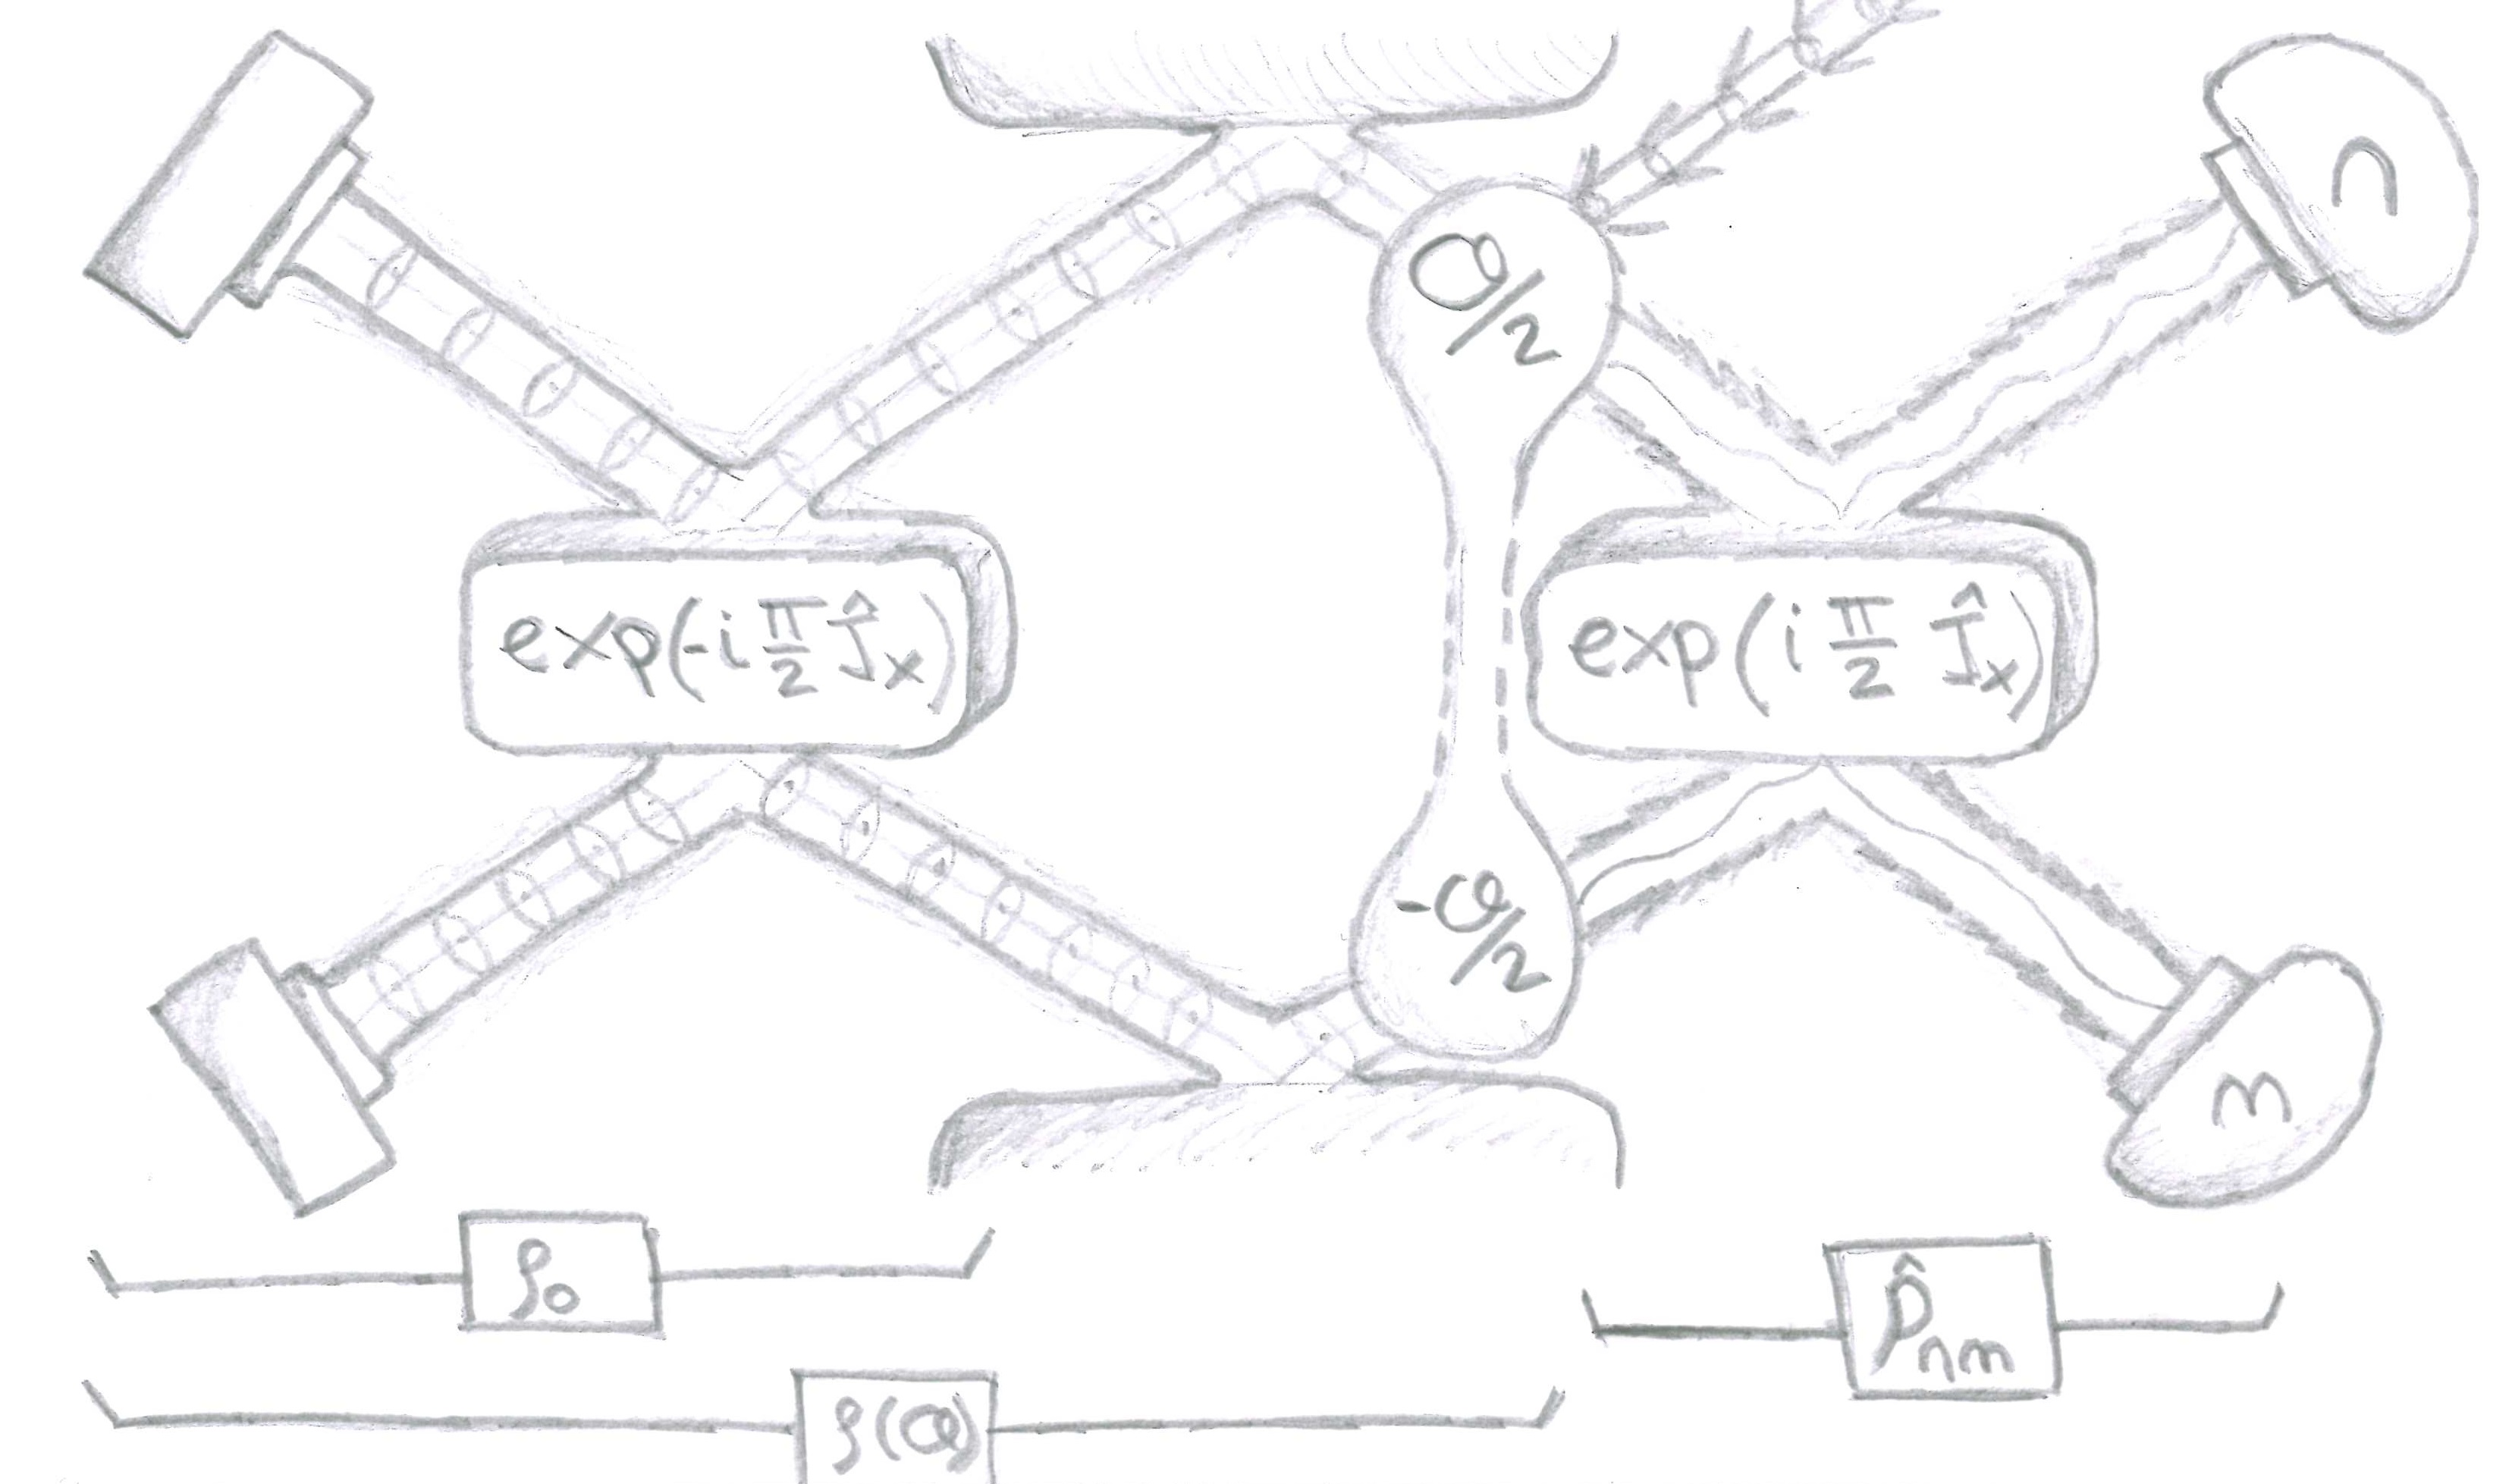
\includegraphics[trim={0cm 0cm 0cm 0.25cm},clip,width=12cm]{pictures/ch2_fig1}
    \caption[Artistic representation of the Mach-Zehnder interferometer]{Artistic representation of the Mach-Zehnder interferometer. A probe state $\rho_0$ is first prepared by mixing two light beams with a $50$:$50$ beam splitter. Then the probe interacts with an external entity whose properties we wish to study, so that an unknown parameter $\theta$ that is related to them is encoded as $\rho(\theta)$. Finally, the light beams are recombined with a second beam splitter and the number of clicks of each detector are measured. The information about the parameter can be extracted by processing these data.}
    \label{mzinterferometer}
\end{figure}

As a generalisation of the previous idea we can consider two-mode interferometry protocols based on the sequence
\begin{equation}
\rho_0 \rightarrow \mathrm{e}^{-iJ_z\theta} \rightarrow E(m),
\label{mzgeneral}
\end{equation}
for some state $\rho_0$ and POM $E(m)$. This generalised Mach-Zehnder interferometer\footnote{Importantly, the model in equation (\ref{mzgeneral}) is a direct representation of realistic experiments when either $[\rho_0, N_T] = 0$ or $[E(m), N_T] = 0$, or both, where $N_T = a_1^\dagger a_1 + a_2^\dagger a_2$ is the total number operator \cite{yurke1986, pezze2015}. If this is not the case, then the $SU(2)$ symmetry is not satisfied in practice because a second parameter is imprinted by $N_T$ in the transformed probe \cite{pezze2015}. Here we assume that the experiment has been calibrated such that this parameter can be set to zero whenever the previous conditions are not fulfilled, and we consider that only the resources that enter into the scheme once it has been calibrated are relevant \cite{proctor2017networked}.} is the model that we will employ in chapters \ref{chap:nonasymptotic} and \ref{chap:limited} to study single-parameter estimation problems. 

Although the full development of estimation techniques will be carried in the next chapter, let us consider here a simple estimation strategy to illustrate how an interferometer can be used to extract information about $\theta$, as well as to introduce those concepts that play a crucial role in optical interferometry. In particular, suppose that the scheme in equation (\ref{mzgeneral}) is initialised in the pure state $ \rho_0 = \ketbra{\psi_0}$ and that we measure the observable $M = \int dm\,m \ketbra{m}$, recording the outcome $m$. If we repeat this protocol $\mu$ times and $\mu \gg 1$, then in practice we may assume that 
\begin{equation}
\frac{1}{\mu}\sum_{i=1}^\mu m_i \approx \langle \psi_0 | U(\theta)^\dagger M U(\theta) |\psi_0 \rangle = \langle \psi_0 | M(\theta) |\psi_0 \rangle = \langle  M(\theta) \rangle
\end{equation}
due to the law of large numbers, where $M(\theta) = U(\theta)^\dagger M U(\theta)$ and we have introduced the notation $\langle \psi_0 |\Box | \psi_0 \rangle = \langle \Box \rangle$.

Next we observe that while $\mu^{-1}\sum_{i=1}^\mu m_i$ is empirically determined, $\langle M(\theta)\rangle$ is a function of $\theta$ that can be calculated from the theory. Let us further imagine that, according to our prior information, $\theta$ is very close to some known value $\theta'$. In that case we can calculate the Taylor expansion of $\langle M(\theta) \rangle$ and assume that
\begin{equation}
\frac{1}{\mu}\sum_{i=1}^\mu m_i \approx \langle M(\theta') \rangle + \frac{d \langle M(\theta') \rangle}{d\theta}(\theta - \theta'),
\end{equation}
which gives us an estimate for the unknown value if we solve it as an equation for $\theta$.

Finally, given that the relationship between the average $\langle M(\theta)\rangle$ and the parameter $\theta$ is approximately linear, to a good approximation we can connect their uncertainties via the error propagation formula \citep{yurke1986, rafal2015, HofmannHolger2009}
\begin{equation}
\Delta \theta^2 \approx \frac{\Delta M(\theta)^2}{\abs{d\langle M(\theta) \rangle/d\theta}^2},
\label{errorprop}
\end{equation}
where $\Delta M(\theta)^2 = \langle  M(\theta)^2 \rangle - \langle M(\theta)  \rangle^2$. Thus we can use equation (\ref{errorprop}) to quantify the quality of our estimation. 

This simple estimation technique shows in a particularly transparent way how the assumptions of having an abundance of measurement data and a good prior knowledge can enter in quantum metrology protocols. In chapter \ref{chap:methodology} we perform a detailed analysis of these restrictions, and the results in this thesis will demonstrate that the methods that we have proposed open the door to design practical schemes beyond such limitations. 

Despite these difficulties, equation (\ref{errorprop}) can still be useful. On the one hand, this uncertainty can always be accessed experimentally and employed as a measure of sensitivity (see, e.g., \cite{baumgart2016}), since the law of large numbers also implies that
\begin{equation}
\Delta M(\theta)^2 \approx \frac{1}{\mu}\sum_{i=1}^\mu m_i^2 - \left(\frac{1}{\mu}\sum_{i=1}^\mu m_i \right)^2
\end{equation} 
when $\mu$ is large, and $d\langle M(\theta) \rangle/d\theta$ can be approximated by a known constant in the regime that we are considering. On the other hand, equation (\ref{errorprop}) provides a theoretical method to compare the efficiency of different quantum strategies. 

Furthermore, by combining equation (\ref{errorprop}) with the generalised Mandelstam-Tamm uncertainty relation $2 \Delta J_z \Delta M(\theta) \geqslant \abs{d \langle M(\theta)\rangle/d \theta}$ \cite{HofmannHolger2009} we find the quantum Cram\'{e}r-Rao bound for pure states \cite{HofmannHolger2009}
\begin{equation}
\frac{\Delta M(\theta)^2}{\abs{d\langle M(\theta) \rangle/d\theta}^2} \geqslant \frac{1}{4\Delta J_z^2}.
\label{simpleqcrb}
\end{equation}
This result indicates that the sensitivity improves when $4\Delta J_z^2$ increases, and how this is to be achieved can be revealed if we rewrite such quantity as \cite{sahota2015}
\begin{equation}
4\Delta J_z^2 = \bar{n}_1\left( 1 + \mathcal{Q}_1 \right) + \bar{n}_2\left( 1 + \mathcal{Q}_2 \right) - 2\mathcal{J}\sqrt{\bar{n}_1\bar{n}_2\left( 1 + \mathcal{Q}_1 \right)\left( 1 + \mathcal{Q}_2 \right)},
\label{fishercorrelations}
\end{equation}
where $\bar{n}_i = \langle a_i^\dagger a_i \rangle$ is the mean number of quanta sent through the $i$-th port, 
\begin{equation}
\mathcal{Q}_i = \frac{1}{\bar{n}_i}\left[\langle (a_i^\dagger a_i)^2 \rangle - \bar{n}_i\left(\bar{n}_i+ 1\right)\right]
\end{equation}
is the Mandel $\mathcal{Q}$-parameter that quantifies the photon correlations within the $i$-th mode, and
\begin{equation}
\mathcal{J} = \frac{\langle a_1^\dagger a_1 a_2^\dagger a_2 \rangle - \bar{n}_1\bar{n}_2}{\Delta(a_1^\dagger a_1) \Delta(a_2^\dagger a_2)}
\end{equation}
is a parameter quantifying the correlations between modes. Indeed equation (\ref{fishercorrelations}) shows that we can enhance the sensitivity by either increasing $\mathcal{Q}_i$ or making $\mathcal{J}$ negative, or both. 

These expressions can be further simplified when we consider the important family of path-symmetric probes introduced by Hofmann \cite{HofmannHolger2009}, which is precisely the class of schemes that we will exploit. Following the characterisation given by Sahota and Quesada \cite{sahota2015}, we say that a state is path-symmetric when the conditions
\begin{equation}
\bar{n}_1 = \bar{n}_2 \equiv \bar{n}/2, ~~ \langle (a_1^\dagger a_1)^2\rangle = \langle (a_2^\dagger a_2)^2\rangle
\end{equation}
are satisfied. In that case we have that 
\begin{equation}
4\Delta J_z^2 = \bar{n}(1+\mathcal{Q})(1-\mathcal{J}),
\label{fishercorrpathsym}
\end{equation}
where the parameters quantifying correlations have become
\begin{align}
\mathcal{Q} &= \frac{1}{2\bar{n}}\left[4\langle (a_1^\dagger a_1)^2 \rangle - \bar{n}\left(\bar{n} + 2\right)\right] = \frac{1}{2\bar{n}}\left[4\langle (a_2^\dagger a_2)^2 \rangle - \bar{n}\left(\bar{n} + 2\right)\right],
\nonumber \\
\mathcal{J} &= \frac{\langle a_1^\dagger a_1 a_2^\dagger a_2 \rangle - \bar{n}^2/4}{\Delta(a_1^\dagger a_1)^2}  = \frac{\langle a_1^\dagger a_1 a_2^\dagger a_2 \rangle - \bar{n}^2/4}{\Delta(a_2^\dagger a_2)^2}.
\label{correlationsintro}
\end{align}

Given the nature of $\mathcal{Q}$ and $\mathcal{J}$, from now on we will refer to the former as the amount of \emph{intra-mode correlations}, while the latter will be understood as quantifying \emph{inter-mode correlations} \cite{knott2016local, proctor2017networked}. These are the type of correlations that will be relevant for our analysis of interferometric schemes. 

\subsection{Multi-parameter protocols}
\label{subsec:multischemes}

Single-parameter protocols such as the Mach-Zehnder interferometer provide a simple and intuitive formalism to understand the fundamental limits that nature imposes on our estimation strategies. However, real-world applications typically give rise to estimation problems with several unknown pieces of information. For instance, we may need to determine the range and velocity of a moving object \cite{zhuang2017}, quantify phases and phase diffusion \cite{vidrighin2014, szczykulska2017}, reconstruct an image \cite{humphreys2013, knott2016local, zhang_lu2017}, estimate the components of a field \cite{baumgratz2016}, assess the spatial deformations of a grid of sources \cite{jasminder2016, jasminder2018} or implement distributed sensing protocols using quantum networks \cite{proctor2017networked, proctor2017networkedshort, ge2018, eldredge2018, altenburg2018, qian2019}. For that reason, the second part of this thesis will be dedicated to the study of multi-parameter schemes. 

Our starting point is the general framework for \emph{quantum sensing networks} introduced by Proctor \emph{et al.} \cite{proctor2017networked}. This is a model for spatially distributed sensing, where in general there will be several sets of unknown parameters, and each set will be encoded locally in a sensor. The importance of this configuration is that it allows us to investigate whether the estimation of such parameters can be enhanced by exploiting inter-sensor and intra-sensor correlations \cite{proctor2017networked, proctor2017networkedshort, sammy2016compatibility, eldredge2018, ge2018}, which in a sense generalise the analogous notions for the Mach-Zehnder interferometer \cite{proctor2017networked, knott2016local}. 

Here we focus on a particular subset of the problems that this formalism can accommodate. In particular, we will consider schemes with a single parameter encoded in each sensor, and possibly including an ancillary system. The fact that the sensors are spatially distributed is imposed by means of the local unitary encoding
\begin{equation}
U(\boldsymbol{\theta}) = \mathbb{I}\otimes U_1(\theta_1)\otimes \cdots \otimes U_d(\theta_d),
\label{distsensing}
\end{equation}
while both the state $\rho_0$ and the measurement $E(m)$, which are defined on the same space that $U(\boldsymbol{\theta})$ is, can be correlated with respect to different sensors. Within this framework, we examine two cases. 

In chapters \ref{chap:networks} and \ref{chap:multibayes} we explore the role of inter-sensor correlations in a network designed to estimate local or global properties in the presence of different amounts of data. Each sensor is modelled as a qubit and no ancillary system is assumed, which implies that, in this case, the first component of the partition in equation (\ref{distsensing}) is absent. This scheme could be implemented, for example, with atoms (see section \ref{subsec:qapp} and \cite{proctor2017networked}).

\begin{figure}[t]
\centering
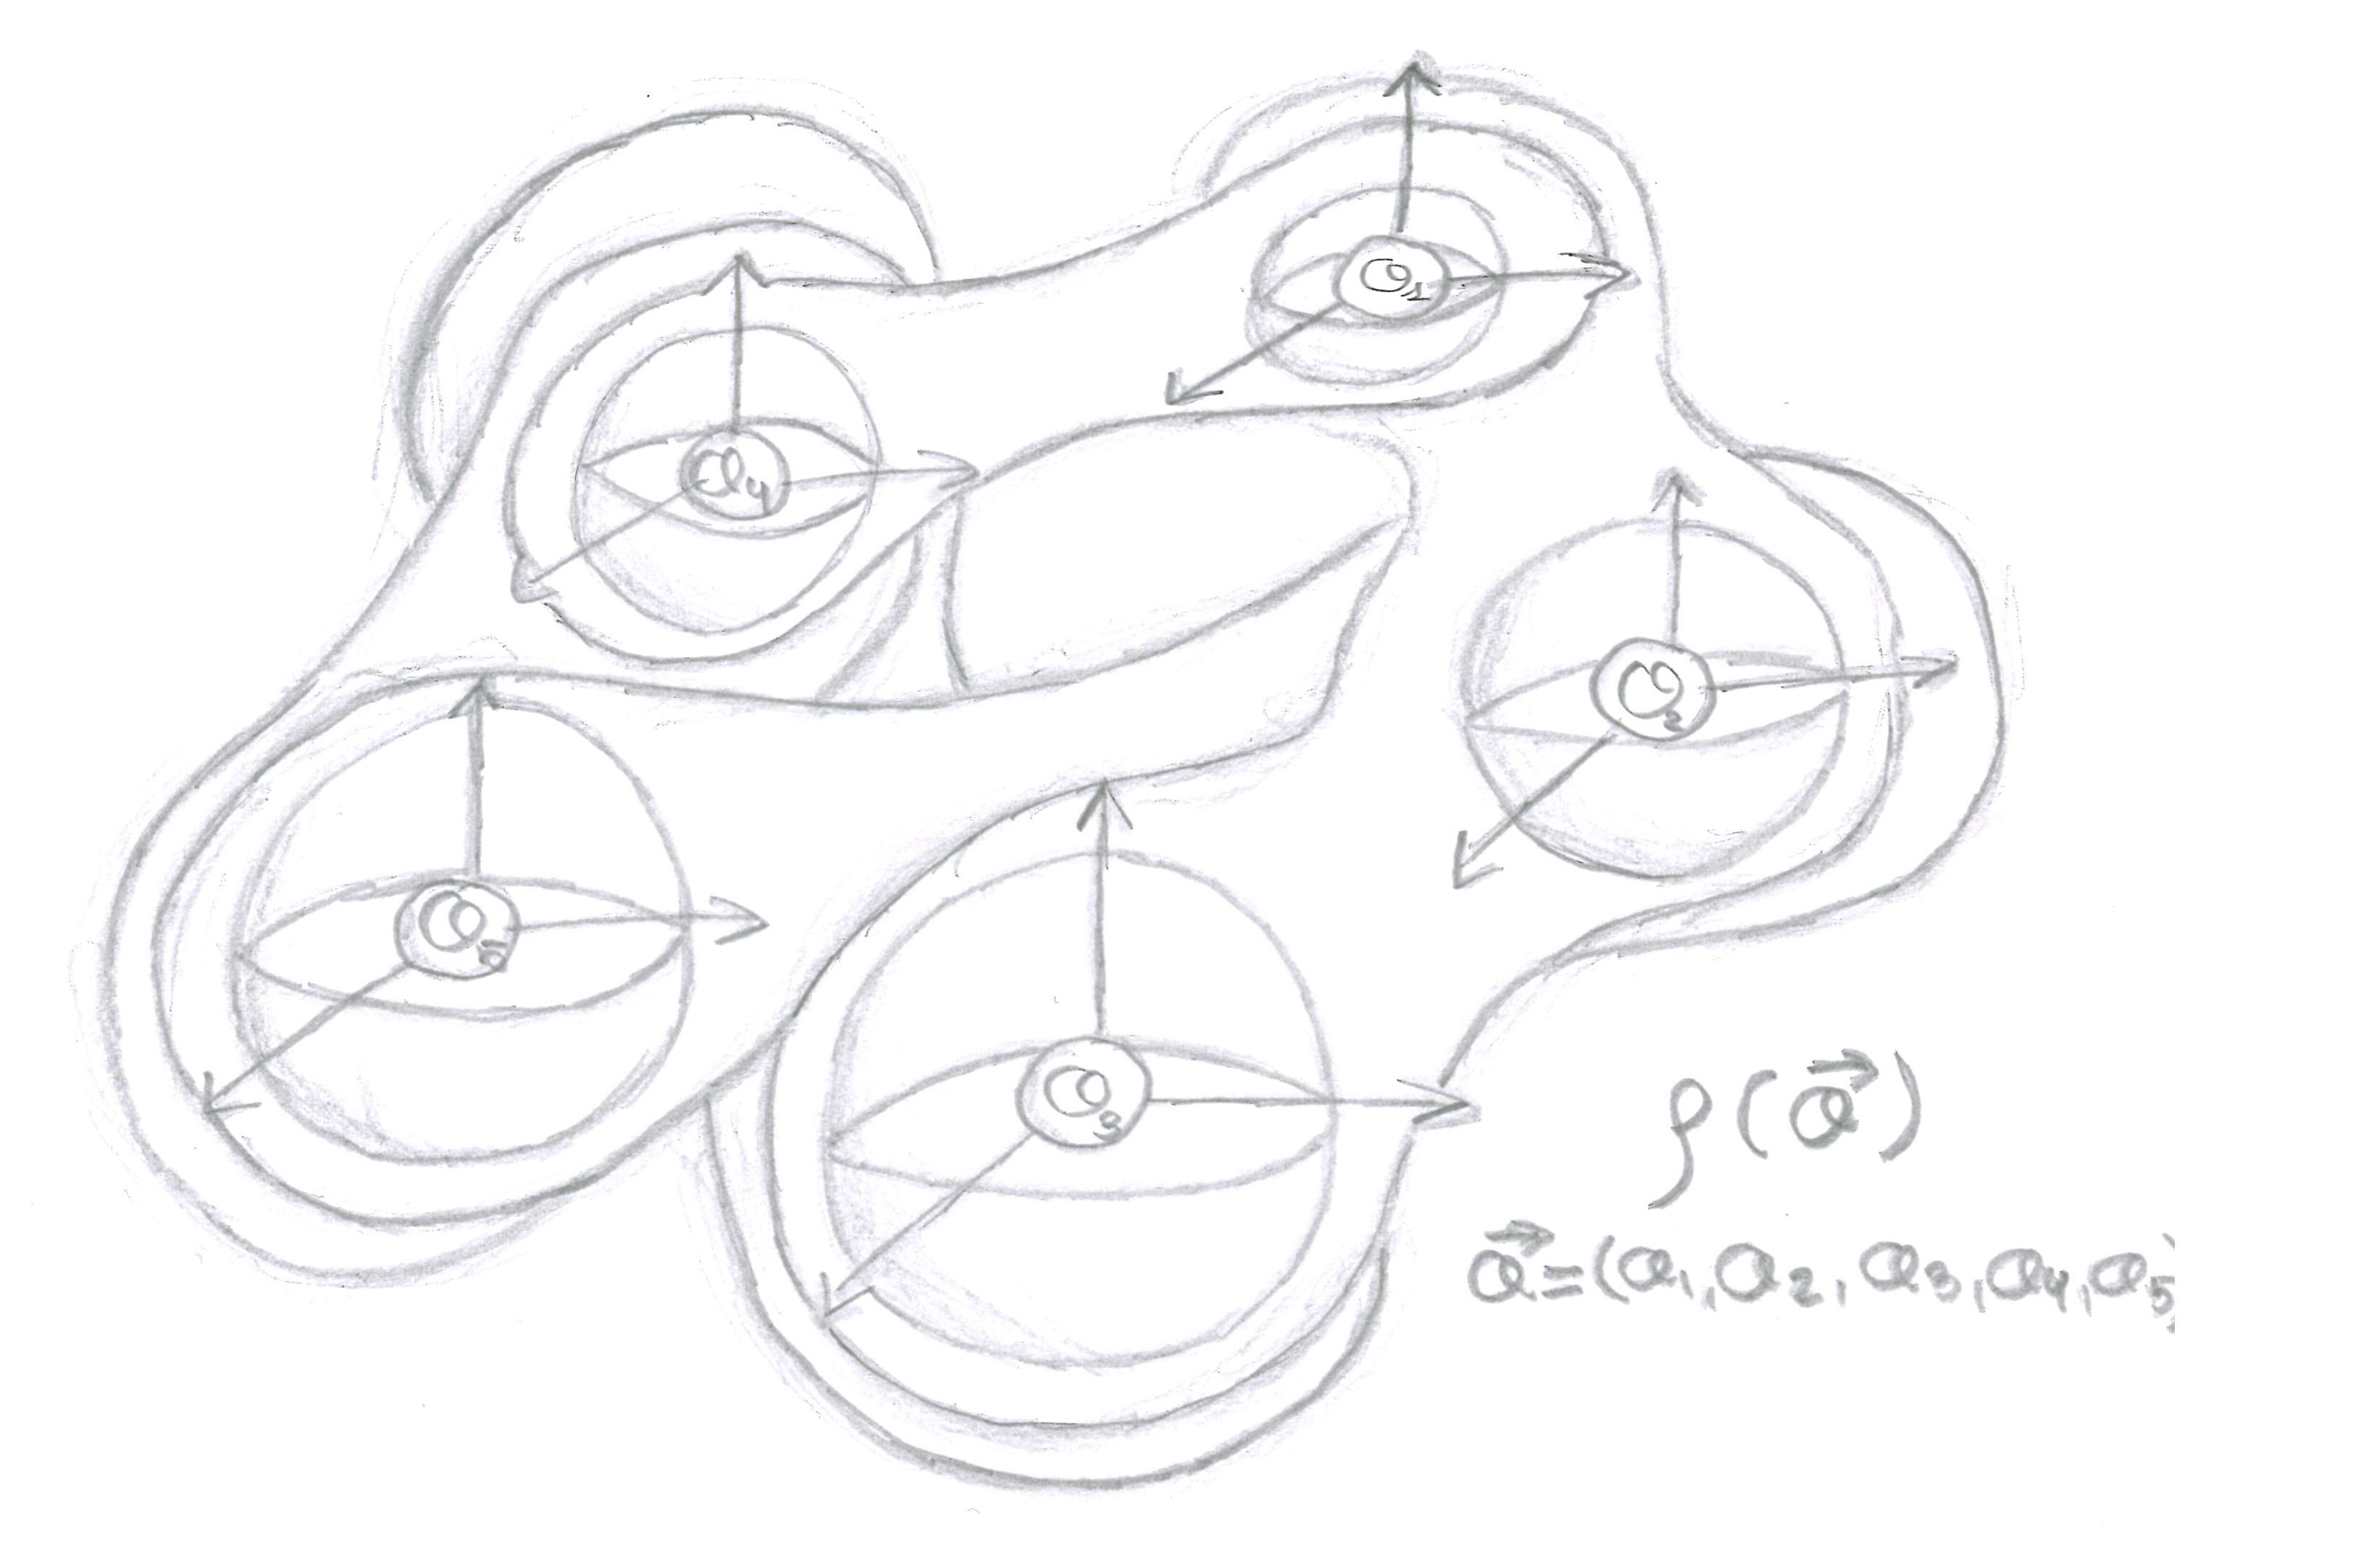
\includegraphics[trim={0cm 0.5cm 0cm 0.25cm},clip,width=14cm]{pictures/ch2_fig2}
\caption[Artistic representation of a quantum sensing network]{Artistic representation of a quantum sensing network. Several qubit sensors are entangled to estimate a set of unknown parameters, which are encoded in the transformed probe $\rho(\boldsymbol{\theta}) = U(\boldsymbol{\theta}) \rho_0 U(\boldsymbol{\theta})^\dagger$.}
\end{figure}

On the other hand, in chapter \ref{chap:multibayes} we also examine a network where each sensor is an optical mode encoding an unknown phase shift that we wish to determine, including an extra mode that acts as a phase reference and whose phase is assumed to be known from the calibration of the experiment\footnote{Counting the resources of this extra beam is motivated when we wish to entangle it with the rest of the network because entangled states are generally difficult to prepare in the laboratory \cite{proctor2017networked}. As with the Mach-Zehnder interferometer, we assume any extra resources that may be needed to calibrate the experiment such that this model applicable in practice \cite{jarzyna2012, proctor2017networked}.} \cite{proctor2017networked}. Therefore, this also fulfils the condition for distributed sensing in equation (\ref{distsensing}). This arrangement encompasses an important imagining protocol that has been extensively studied both with Bayesian \cite{chiara2003, spagnolo2012} and non-Bayesian tools \cite{spagnolo2012, humphreys2013}, and that has produced a rich literature about the potential enhancement that the global estimation of several parameters might provide, or the lack of it \cite{humphreys2013, knott2016local, proctor2017networked, proctor2017networkedshort, altenburg2018}. This protocol is one of the possible ways in which we can generalise two-mode interferometry to the multi-parameter case. For an alternative generalisation where each sensor is a full interferometer, see \cite{knott2016local}.

It is important to note that existing literature employs the notions of \emph{local} and \emph{global} estimation strategies in two different ways. Within the context of this section, a strategy is said to be local if neither the state nor the measurement present correlations with respect to the partition in equation (\ref{distsensing}), and global otherwise. That is, a local strategy is uncorrelated according to the definitions in section \ref{subsec:qapp}. However, if instead we focus on the more general context of estimation theory, local strategies are those that rely on a high amount of prior knowledge about the parameters of interest, while a global estimation refers to situations where we are almost completely ignorant about them. In the next chapter we will see that our protocols will be designed to operate in the intermediate regime between the two latter extremes. The exact meaning that the terms \emph{local} and \emph{global} have in each situation will be clear from the context.   

\section{Chapter summary}

The formalism reviewed in this chapter enables us to perform three tasks that are crucial for the development of quantum metrology: representing information, encoding it in quantum systems, and manipulating those systems to extract such information, which is the final goal.

We have seen that the uncertain information associated with natural phenomena can be suitably modelled with the objective version of Bayesian probability theory. The importance of this fact will become apparent once we have introduced the condition of limited data in our estimation protocols. Moreover, this perspective has offered a clear intuition to understand the empirical link between our probability models and the relative frequencies that we measure in the laboratory, as well as their conceptual differences. Crucially, this link plays a fundamental role in verifying the validity of quantum predictions.

On the other hand, we have revisited the foundations of quantum mechanics to understand the reasons behind the success of quantum technologies in general, and of quantum metrology in particular. The key observation is that while the existence of the quantum of action constrains the probability models that we can construct, we also have freedom to choose the functions of dynamical variables that give rise to states and measurements. Hence, the combination of both features provides us with a framework that is more realistic than the classical paradigm and flexible enough to develop new applications on the basis of quantum entities.

As a final step we have described two important classes of quantum schemes: a generalised version of the Mach-Zehnder interferometer and a quantum sensing network model for distributed sensing, and we have identified the types of correlations that may be present in these systems as one of the fundamental features to be exploited in our study of quantum metrology protocols. 